

\documentclass[10pt, conference, compsocconf]{IEEEtran}

\usepackage{graphicx}
\usepackage{algorithmic,listings}
\lstset{language=C,basicstyle=\small\ttfamily, basewidth=0.51em}
\usepackage{url}
\usepackage{tabularx}
\usepackage{subfig}
\usepackage{float}
\usepackage{underscore}
% correct bad hyphenation here
\hyphenation{op-tical net-works semi-conduc-tor}

\graphicspath{{figures/}}
\pagestyle{plain}
\begin{document}


\title{Application-Level Regression Testing Framework using Jenkins}


% author names and affiliations
% use a multiple column layout for up to two different
% affiliations


% conference papers do not typically use \thanks and this command
% is locked out in conference mode. If really needed, such as for
% the acknowledgment of grants, issue a \IEEEoverridecommandlockouts
% after \documentclass

% for over three affiliations, or if they all won't fit within the width
% of the page, use this alternative format:
%
\author{\IEEEauthorblockN{Author1, Timothy Bouvet, Galen Arnold}
%xxxx\IEEEauthorrefmark{3} and
%xxxx\IEEEauthorrefmark{4}}
%\IEEEauthorblockA{\IEEEauthorrefmark{1}National Institute for Computational Science\\
National Institute for Computational Sciences\\
The University of Tennessee, Knoxville, TN 37996\\
\{email1,tbouvet@illinois.edu,gwarnold@illinois.edu\}@domain.edu}
%\IEEEauthorblockA{\IEEEauthorrefmark{4}Electrical Engineering and Computer Science Department\\University of Tennessee, Knoxville, TN 37996\\xx@eecs.utk.edu}
%}


% use for special paper notices
%\IEEEspecialpapernotice{(Invited Paper)}



% make the title area
\maketitle
\thispagestyle{plain}

\begin{abstract}
This paper will explore the challenges of regression testing and monitoring of large scale systems such as NCSA’s Blue Waters. Our goal was to come up with an automated solution for running user-level regression tests to evaluate system usability and performance. Another requirement was to find an automated solution for running a suite of test jobs that reveal the system health after upgrades and outages before returning the system to service. We evaluated test frameworks such as Inca [1] and Jenkins [2]. Jenkins was chosen for its versatility, large user base, and multitudes of plugins including plotting test results over time. We utilize these plots to track trends and alert us to system-level issues before they are reported by our partners (users). Not only does Jenkins have the ability to store historical data but it can also send customized notifications (e.g. send email or text pages) based on the result of a test. Some of the requirements we had include two-factor authentication to access Jenkins GUI with privileges to execute tests and account management through LDAP. In this paper we describe our implementation of these requirements to ensure a secure and usable deployment of a Jenkins instance.

Our Jenkins instance was deployed on a vSphere managed VM running Centos 6.8. Security was of the highest concern since Jenkins has the ability to execute commands on our login nodes. Jenkins is set to log in as a standard user account with passwordless access (commands to the login nodes can be input via Jenkins GUI) using ssh keys scoped to the VM. The VM (bwjenkins) was closely vetted by our security team on our test and development system (TDS) before it was allowed access to Blue Waters. Iptables was used to lock bwjenkins down to a small internal ip space to ensure the highest security. An anonymous user account was enabled with ‘read-only’ access to view current and historical test results. During a test, Jenkins downloads software, builds the software, submits a job, awaits completion, gathers and plots the results or returns error information during a failure. These are full end to end functionality testing of the programming environment, queueing system, license servers and provide historical metrics to quickly detect regressions.

In this paper we describe in detail our challenges and experiences in deploying Jenkins as a user-level system-wide regression testing and monitoring framework for Blue Waters. We will also show some application-based system-level tests we have implemented in Jenkins and share results of those tests. The deployment of Jenkins allow us to monitor and detect issues as early as possible from the perspective of a user on Blue Waters, eventually providing a more efficient service for better user experience.
\end{abstract}

\begin{IEEEkeywords}
Performance; Benchmarking; Computer architecture
\end{IEEEkeywords}


% For peer review papers, you can put extra information on the cover
% page as needed:
% \ifCLASSOPTIONpeerreview
% \begin{center} \bfseries EDICS Category: 3-BBND \end{center}
% \fi
%
% For peerreview papers, this IEEEtran command inserts a page break and
% creates the second title. It will be ignored for other modes.
\IEEEpeerreviewmaketitle

\section{Motivation}


\begin{lstlisting}[float,frame=tb,captionpos=t,language=bash,caption={Apache Configuration Example}, label=lst:apacheconfig]

# First, we configure the "default" to be a very 
# restrictive set of features.  
#
<Directory />
    Options FollowSymLinks
    AllowOverride None  
</Directory>

\end{lstlisting}

\section{Jenkins Configuration}
\label{sec:JenkinsConfiguration}

\subsection{Introduction to Jenkins}
\subsection{Master-Node Configuration}
\subsection{Accessing Login Nodes}


\section{Authentication and Authorization}
\label{sec:AuthenticationAuthorization}

\subsection{Security Considerations}
Blue Waters is an OTP only restricted access system. Enabling Jenkins access to Blue Waters posed some unique security hurdles that we had to overcome. Jenkins has the ability to execute commands on our login nodes. Jenkins is set to log in as a standard user account with passwordless access (commands to the login nodes can be input via Jenkins GUI) using ssh keys scoped to the VM. We restricting access to the physical VM and Jenkins GUI (bwjenkins) utilizing iptables, SSL and OTP. The VM allows restricted host-based ssh (port 22) access from two secure OTP only administrative systems. The Jenkins GUI presented additional challenges. We setup reverse proxy to run Jenkins behind apache/http with SSL for access to the administrative console. All the configuration is in /etc/httpd/config.d/ssl.conf. An anonymous GUI view was setup (config file snippets below)

\begin{lstlisting}
/etc/ssh/sshd_config:
Match Host bwbh1.ncsa.illinois.edu,
bwbh2.ncsa.illinois.edu
HostbasedAuthentication yes


/etc/sysconfig/iptables:
-A INPUT -s 141.142.0.0/16 -m state --state NEW -m tcp 
-p tcp --dport 22 -j ACCEPT
-A INPUT -s 172.16.0.0/15 -m state --state NEW -m tcp 
-p tcp --dport 22 -j ACCEPT *delete maybe*
-A INPUT  -m state --state NEW -m tcp -p tcp --dport 80 
-j ACCEPT
-A INPUT -s 141.142.0.0/16 -m state --state NEW -m tcp 
-p tcp --dport 443 -j ACCEPT

/etc/httpd/config.d/ssl.conf:
Listen 443
<VirtualHost _default_:443>
SSLSessionCache         shmcb:/var/cache/mod_ssl/scache
(512000) Reuben how you cache the opt?
SSLSessionCacheTimeout  300
ServerName bwjenkins.ncsa.illinois.edu:443
 # -- The following sets ReverseProxy for Jenkins
  ProxyRequests       Off
  ProxyPreserveHost   On
  AllowEncodedSlashes On
  <Proxy *>
    Order deny,allow
    Allow from all
  </Proxy>
  ProxyPass       / http://localhost:8080/ nocanon
  ProxyPassReverse / http://localhost:8080/
  ProxyPassReverse / http://bwjenkins.ncsa.illinois.edu/
  RequestHeader set X-Forwarded-Proto "https"
  RequestHeader set X-Forwarded-Port "443"

  DefineExternalAuth pwauth+session pipe /usr/local/bin/
  pwauth+session
  <LocationMatch / > 
    AuthType Basic
    AuthBasicProvider external
    AuthName "NCSA RSA OTP login" 
    AuthExternal pwauth+session
    require valid-user
    
    RequestHeader unset "X-Forwarded-User"
    RequestHeader set "X-Forwarded-User" (REMOTE_USER)

  </LocationMatch>
\end{lstlisting}

\subsection{Configuration Choices}

\section{Anatomy of A Test}
\label{sec:TestAnatomy}


\section{SWTools Integration}
\label{sec:SWToolsIntegration}


\section{Use Cases}
\label{sec:results}
\subsection{IOR Lustre scratch test}
We created Jenkins tests to run the IOR MPI parallel filesystem test to run at a modest scale and validate filesystem functionality and performance for the scratch filesystem on a periodic basis. The test is scaled to provide representative performance numbers for a typical small application while not creating issues with other jobs or the filesystem at large.  One of our best practices is to provide a management level summary description for casual jenkins users who want to view the test but do not need to understand the jenkins configuration and execution details.  
\begin{figure}[H]
\centering
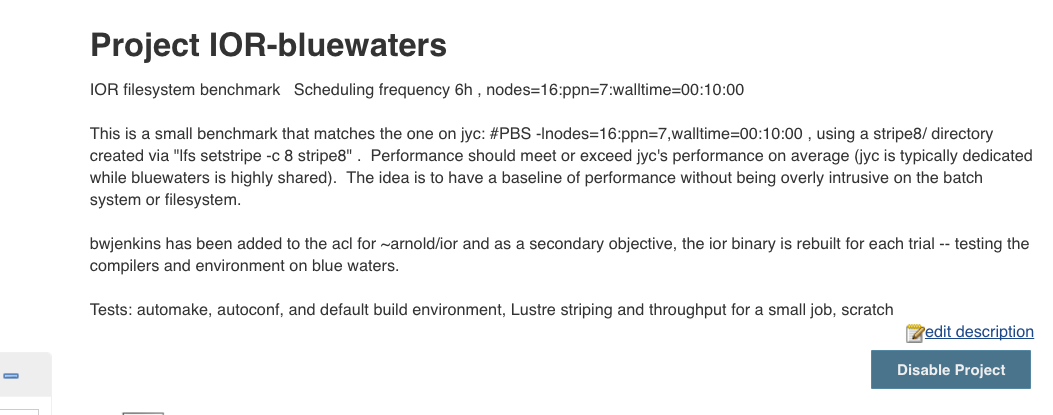
\includegraphics[width=0.5\textwidth]{IOR-bluewaters-descr}
\caption{ IOR description in jenkins }
\label{fig:IOR-bluewaters-descr}
\end{figure}
Where possible, tests build from source and exercise multiple user-facing system components such as: git for external connectivity and loading modules to test the defaults in the environment.  Where scripts on the SSH site are used, they are echoed and/or displayed with "cat -n" to make console output verbose and easy to debug in case of errors.  

\begin{figure}[H]
\centering
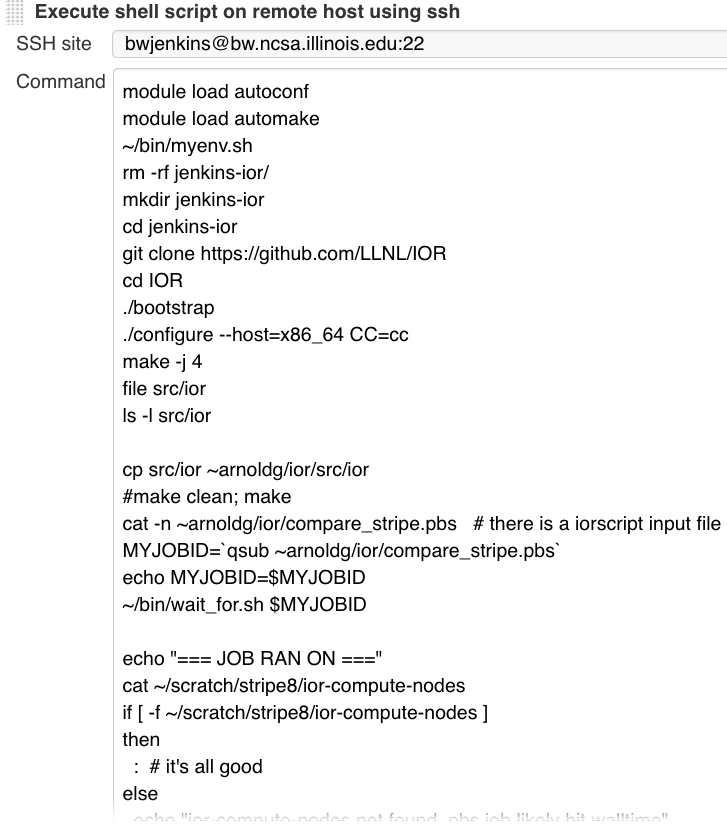
\includegraphics[width=0.5\textwidth]{IOR-configuration-sample}
\caption{ IOR configuration sample }
\label{fig:IOR-configuration-sample}
\end{figure}

The test is set to run as scheduled by Jenkins with a best-effort through our batch system.  The test blocks such that the next test will not start until the previous one has completed.  We employ a watchdog script to block the exit from the test until the batch system marks it as finished.

\begin{lstlisting}[float,frame=tb,captionpos=t,language=bash,caption={pbs/torque watchdog script}, label=lst:watchdog]
#!/bin/bash
echo "=== RUNNING $0 ==="
if [ $# -lt 1 ]
then
  echo "$0: missing argument for jobid"
  exit 1
fi
while true
do
	MYQSTAT=`qstat $1`
	if test "$MYQSTAT" = ""
        then
		echo $1 finished
		exit
	else
		DATE=`date`
		echo "$DATE: waiting for $1 to finish"
	fi
	sleep 5m
done
\end{lstlisting}

\begin{figure}[H]
\centering
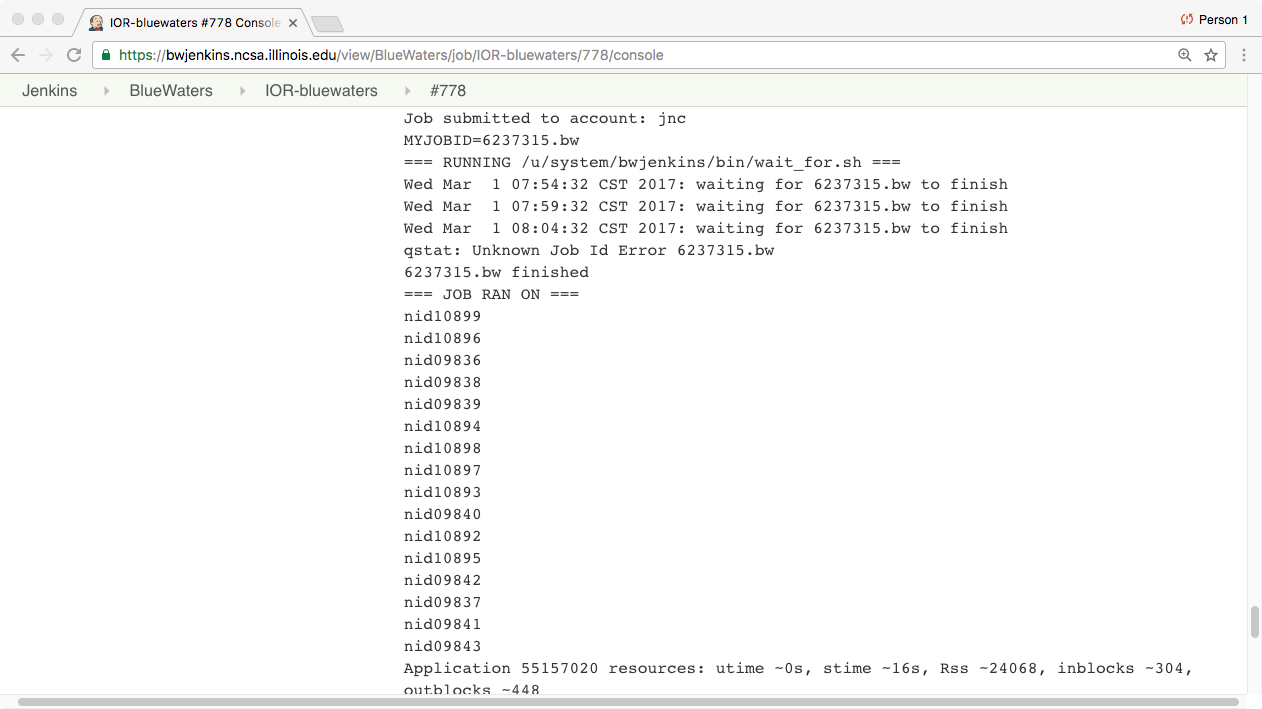
\includegraphics[width=0.5\textwidth]{IOR-watchdog-out}
\caption{ IOR watchdog console output }
\label{fig:IOR-watchdog-out}
\end{figure}
For tests that produce an interesting performance metric like IOR, we save that output to a file and use the Jenkins plotting feature to produce plots. 
\begin{figure}[H]
\centering
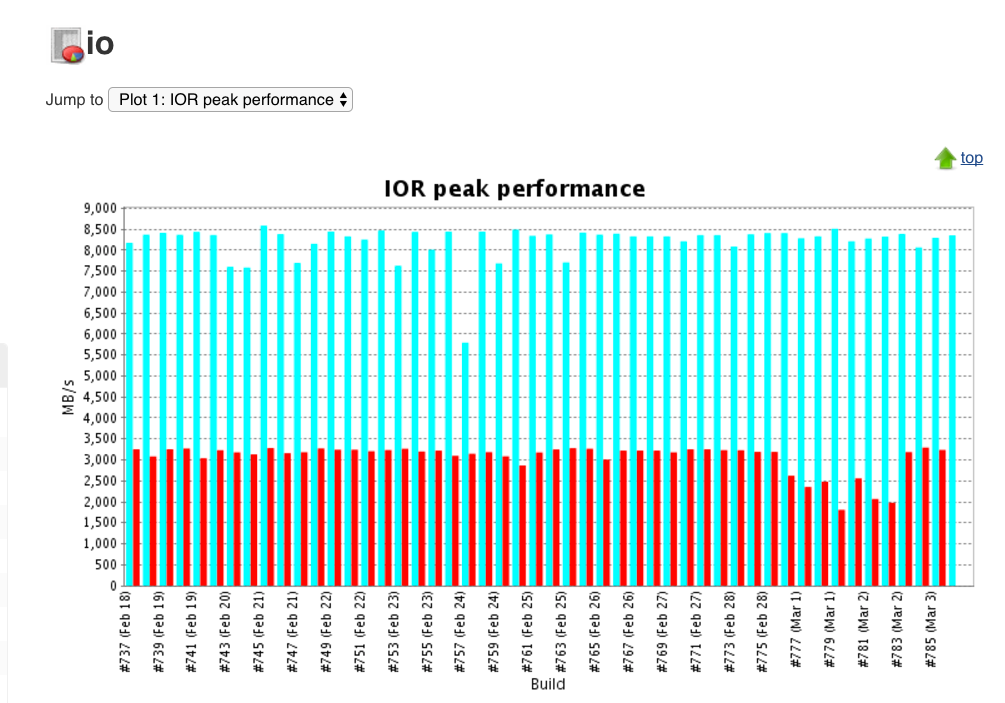
\includegraphics[width=0.5\textwidth]{IOR-plot}
\caption{ IOR plot view }
\label{fig:IOR-plot}
\end{figure}
A plot like this helps us with performance baselines and we can quickly react to changes in the software environment or filesystem configuration.

\subsection{mdtest Lustre tests}
The mdtest metadata test is run on the home and scratch filesystems to validate metadata server performance.  The IOR and mdtest user-facing tests complement the fine-grained detail we are able to glean from the backed system-side counters in our OVIS database where we record details about individual server metrics and network traffic on the Cray Gemini fabric.  
\begin{figure}[H]
\centering
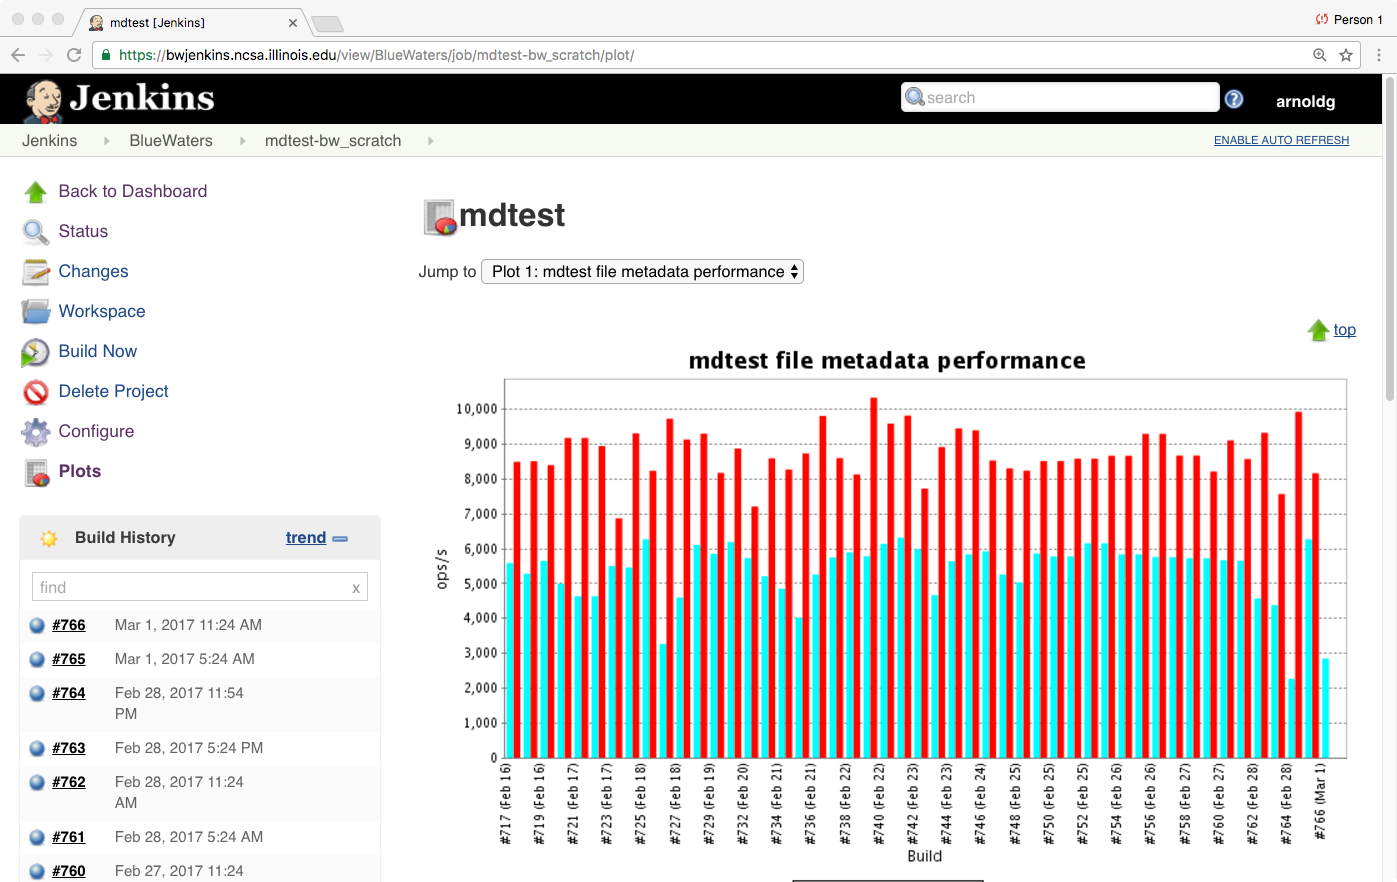
\includegraphics[width=0.5\textwidth]{mdtest-plot}
\caption{ mdtest plot view }
\label{fig:mdtest-plot}
\end{figure}

An additional best practice is to enable E-mail Notifications to the test author and/or other interested parties.  E-mail for unstable builds will cause an E-mail every time the test state changes (from successful to failing and again when back to successful ).
\begin{figure}[H]
\centering
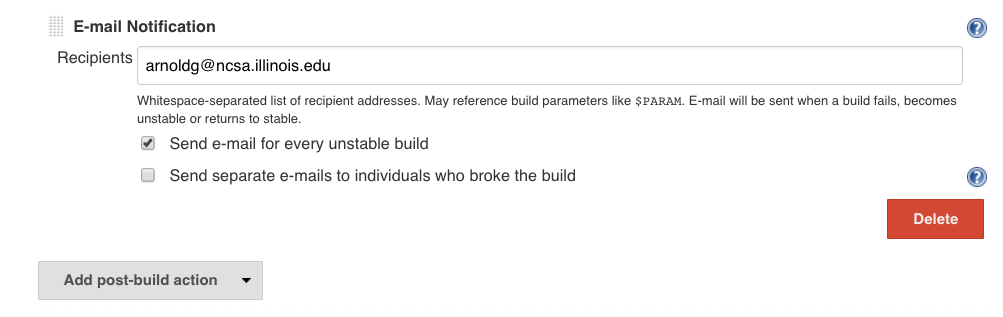
\includegraphics[width=0.5\textwidth]{mdtest-config-email}
\caption{ mdtest email configuration }
\label{fig:mdtest-config-email}
\end{figure}

\subsection{special projects}
The tabs display of our Jenkins instance is used to group tests and we add tabs for special projects.   For example we clone existing tests for evaluating a new software stack on our test login node.   Our test rack has a separate set of tests from our production system and is used as our Jenkins test development area.  The sustained petascale performance benchmarks are in their own tab since they can run at scale and are only run on-demand (not scheduled by Jenkins ).
\begin{figure}[H]
\centering
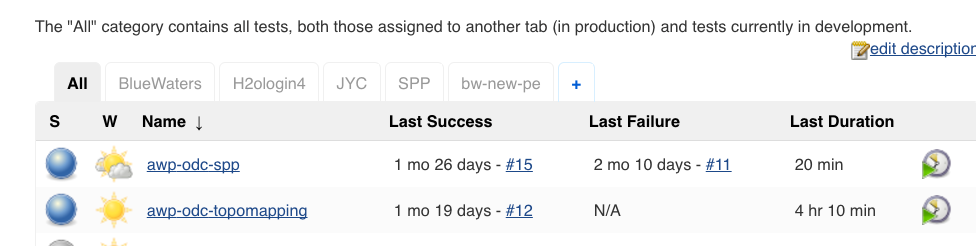
\includegraphics[width=0.5\textwidth]{tabs-display}
\caption{ tabs for project areas }
\label{fig:tabs-display}
\end{figure}

\section{Conclusion}
\label{sec:conclusion}

% use section* for acknowledgement
\section*{Acknowledgment}
This research used resources at the National Institute for Computational Sciences, funded by the National Science Foundation (NSF).

% trigger a \newpage just before the given reference
% number - used to balance the columns on the last page
% adjust value as needed - may need to be readjusted if
% the document is modified later
\IEEEtriggeratref{8}
% The "triggered" command can be changed if desired:
\IEEEtriggercmd{\enlargethispage{-2in}}

% references section

% can use a bibliography generated by BibTeX as a .bbl file
% BibTeX documentation can be easily obtained at:
% http://www.ctan.org/tex-archive/biblio/bibtex/contrib/doc/
% The IEEEtran BibTeX style support page is at:
% http://www.michaelshell.org/tex/ieeetran/bibtex/
%\bibliographystyle{IEEEtran}
% argument is your BibTeX string definitions and bibliography database(s)
%\bibliography{IEEEabrv,../bib/paper}
%
% <OR> manually copy in the resultant .bbl file
% set second argument of \begin to the number of references
% (used to reserve space for the reference number labels box)

%\begin{thebibliography}{9}

%\bibliographystyle{IEEEtran}
%\bibliographystyle{unsrt}
%\bibliography{references}

%\end{thebibliography}

% that's all folks
\end{document}
